\documentclass[12pt,convert={false}]{standalone}
\usepackage[dvipsnames]{xcolor}
\usepackage{tikz}
\usetikzlibrary{shapes,arrows,positioning,calc,patterns,arrows.meta, bending, graphs, shadings,quotes,intersections}
\usetikzlibrary{external}
%\tikzexternalize[prefix=tikz/]
\usepackage{pgfplots}
\pgfplotsset{compat=1.16}
\usepgfplotslibrary{fillbetween}
\begin{document}
 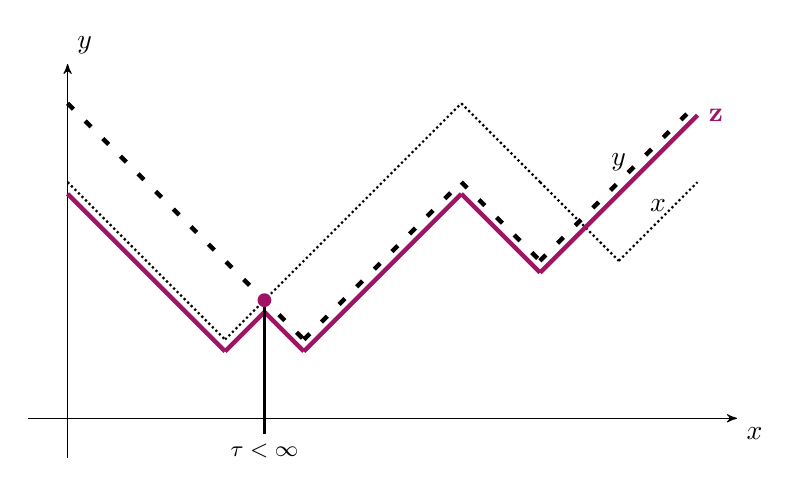
\begin{tikzpicture}[
	>=stealth', axis/.style={->},
	point/.style={circle, inner sep=0pt, fill, minimum size=4pt, label=#1},
	scale=1]
	\draw[axis] (0,-0.5) -- (0,4.5) node[above right]{$y$};
	\draw[axis] (-0.5,0) -- (8.5,0) node[below right]{$x$};
	\draw[loosely dashed, ultra thick, black] (0,4) -- (3,1);
	\draw[loosely dashed, ultra thick, black] (3,1) -- (5,3);
	\draw[loosely dashed, ultra thick, black] (5,3) -- (6,2);
	\draw[loosely dashed, ultra thick, black] (6,2) -- (8,4) node [black,midway,above]{$y$};
	\draw[densely dotted, thick, black] (0,3) -- (2,1);
	\draw[densely dotted, thick, black] (2,1) -- (5,4);
	\draw[densely dotted, thick, black] (5,4) -- (6,3);
	\draw[densely dotted, thick, black] (6,3) -- (7,2);
	\draw[densely dotted, thick, black] (7,2) -- (8,3) node [black,midway,above]{$x$};
	\begin{scope}[shift={(0,-0.15)}]
		\draw[ultra thick, RedViolet] (0,3) -- (2,1);
		\draw[ultra thick, RedViolet] (2,1) -- (2.5,1.5);
		\draw[ultra thick, RedViolet] (2.5,1.5) -- (3,1);
		\draw[ultra thick, RedViolet] (3,1) -- (5,3);
		\draw[ultra thick, RedViolet] (5,3) -- (6,2);
		\draw[ultra thick, RedViolet] (6,2) -- (8,4) node [RedViolet, right]{$\textbf{z}$};
	\end{scope}
	\draw[thick](2.5,-0.2) -- (2.5,1.5);
	\node[below] at (2.5,-0.2) {\footnotesize$\tau<\infty$};
	\node[circle, fill, inner sep=0pt, minimum size=5pt,RedViolet] at (2.5,1.5) {};
\end{tikzpicture}
\end{document}
